% !TEX program = pdflatex

\documentclass[11pt,a4paper]{article}
\usepackage{fullpage}                % See geometry.pdf to learn the layout options. There are lots.
\usepackage[parfill]{parskip}    % Activate to begin paragraphs with an empty line rather than an indent
\usepackage{graphicx}
\usepackage{amssymb}
\usepackage{epstopdf}
\usepackage{hyperref}
\DeclareGraphicsRule{.tif}{png}{.png}{`convert #1 `dirname #1`/`basename #1 .tif`.png}

\title{\TeX Help user guide}
\author{Neil Sims}
\date{\today}                                           % Activate to display a given date or no date


\begin{document}
\maketitle
\section{Initial configuration}
When \TeX Help is run for the first time, it needs to search the help documents that are shipped with the \TeX Live distribution. To do this, select the root folder of the required \TeX Live distribution:

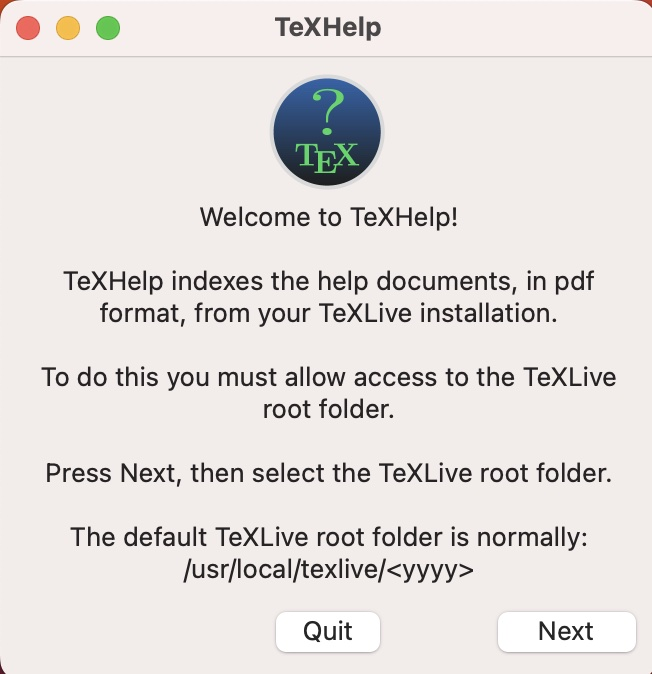
\includegraphics[scale=0.25]{WelcomePage.jpg} 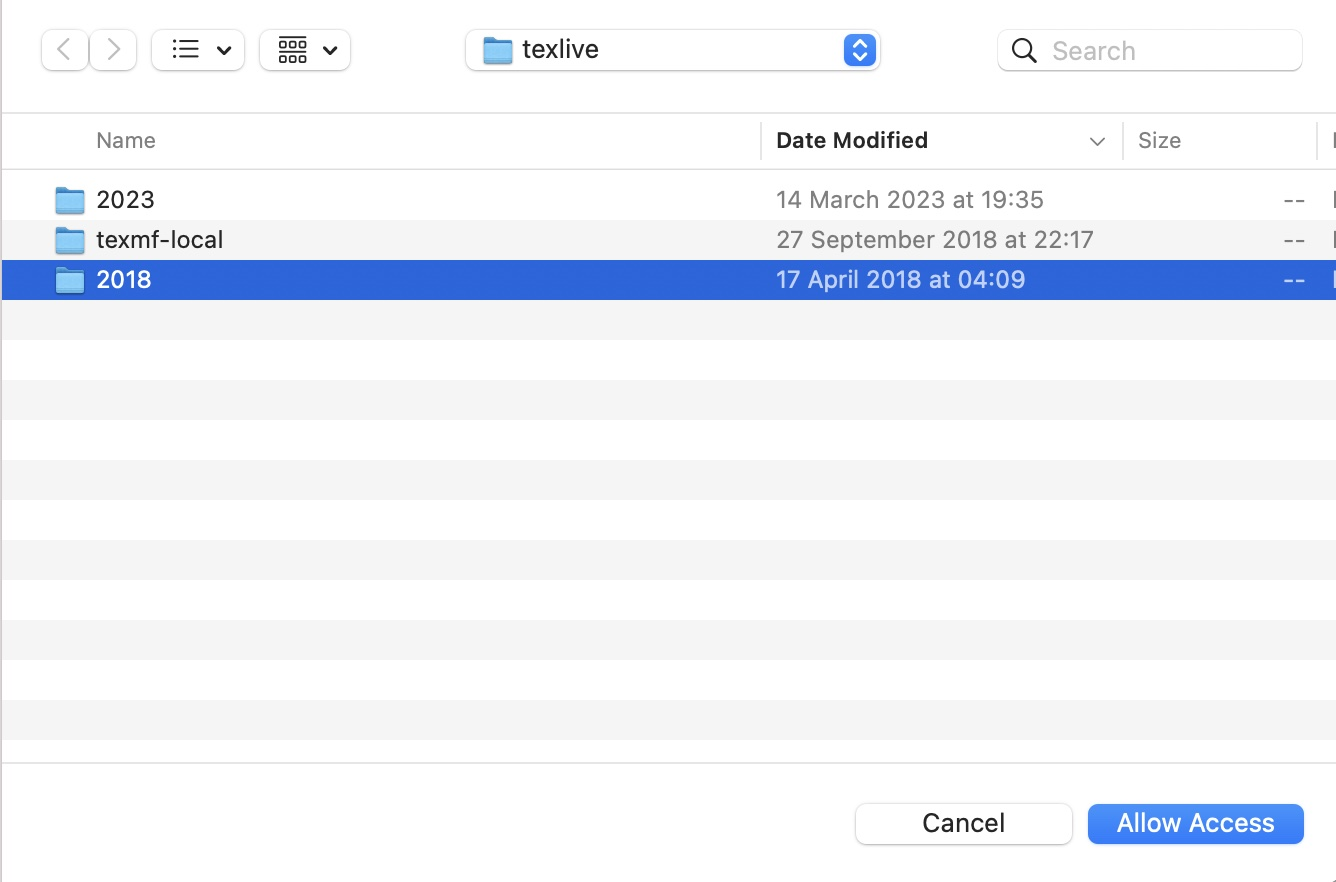
\includegraphics[scale=0.2]{RootFolder.jpg}

If the folder is configured correctly, then the following message appears:

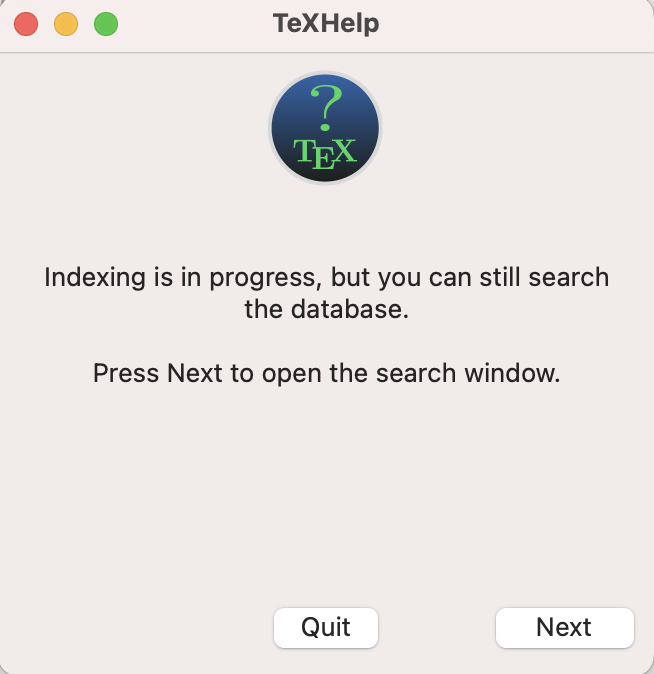
\includegraphics[scale=0.5]{Indexing.png}

Click next and the Advanced Search Pane opens. Indexing can take a few hours.

\section{Advanced Search}

This includes some explanation of how to search, but simple free text search can also be performed. Press enter to perform the search. \textbf{When indexing is running, the search action can take some time to complete}.

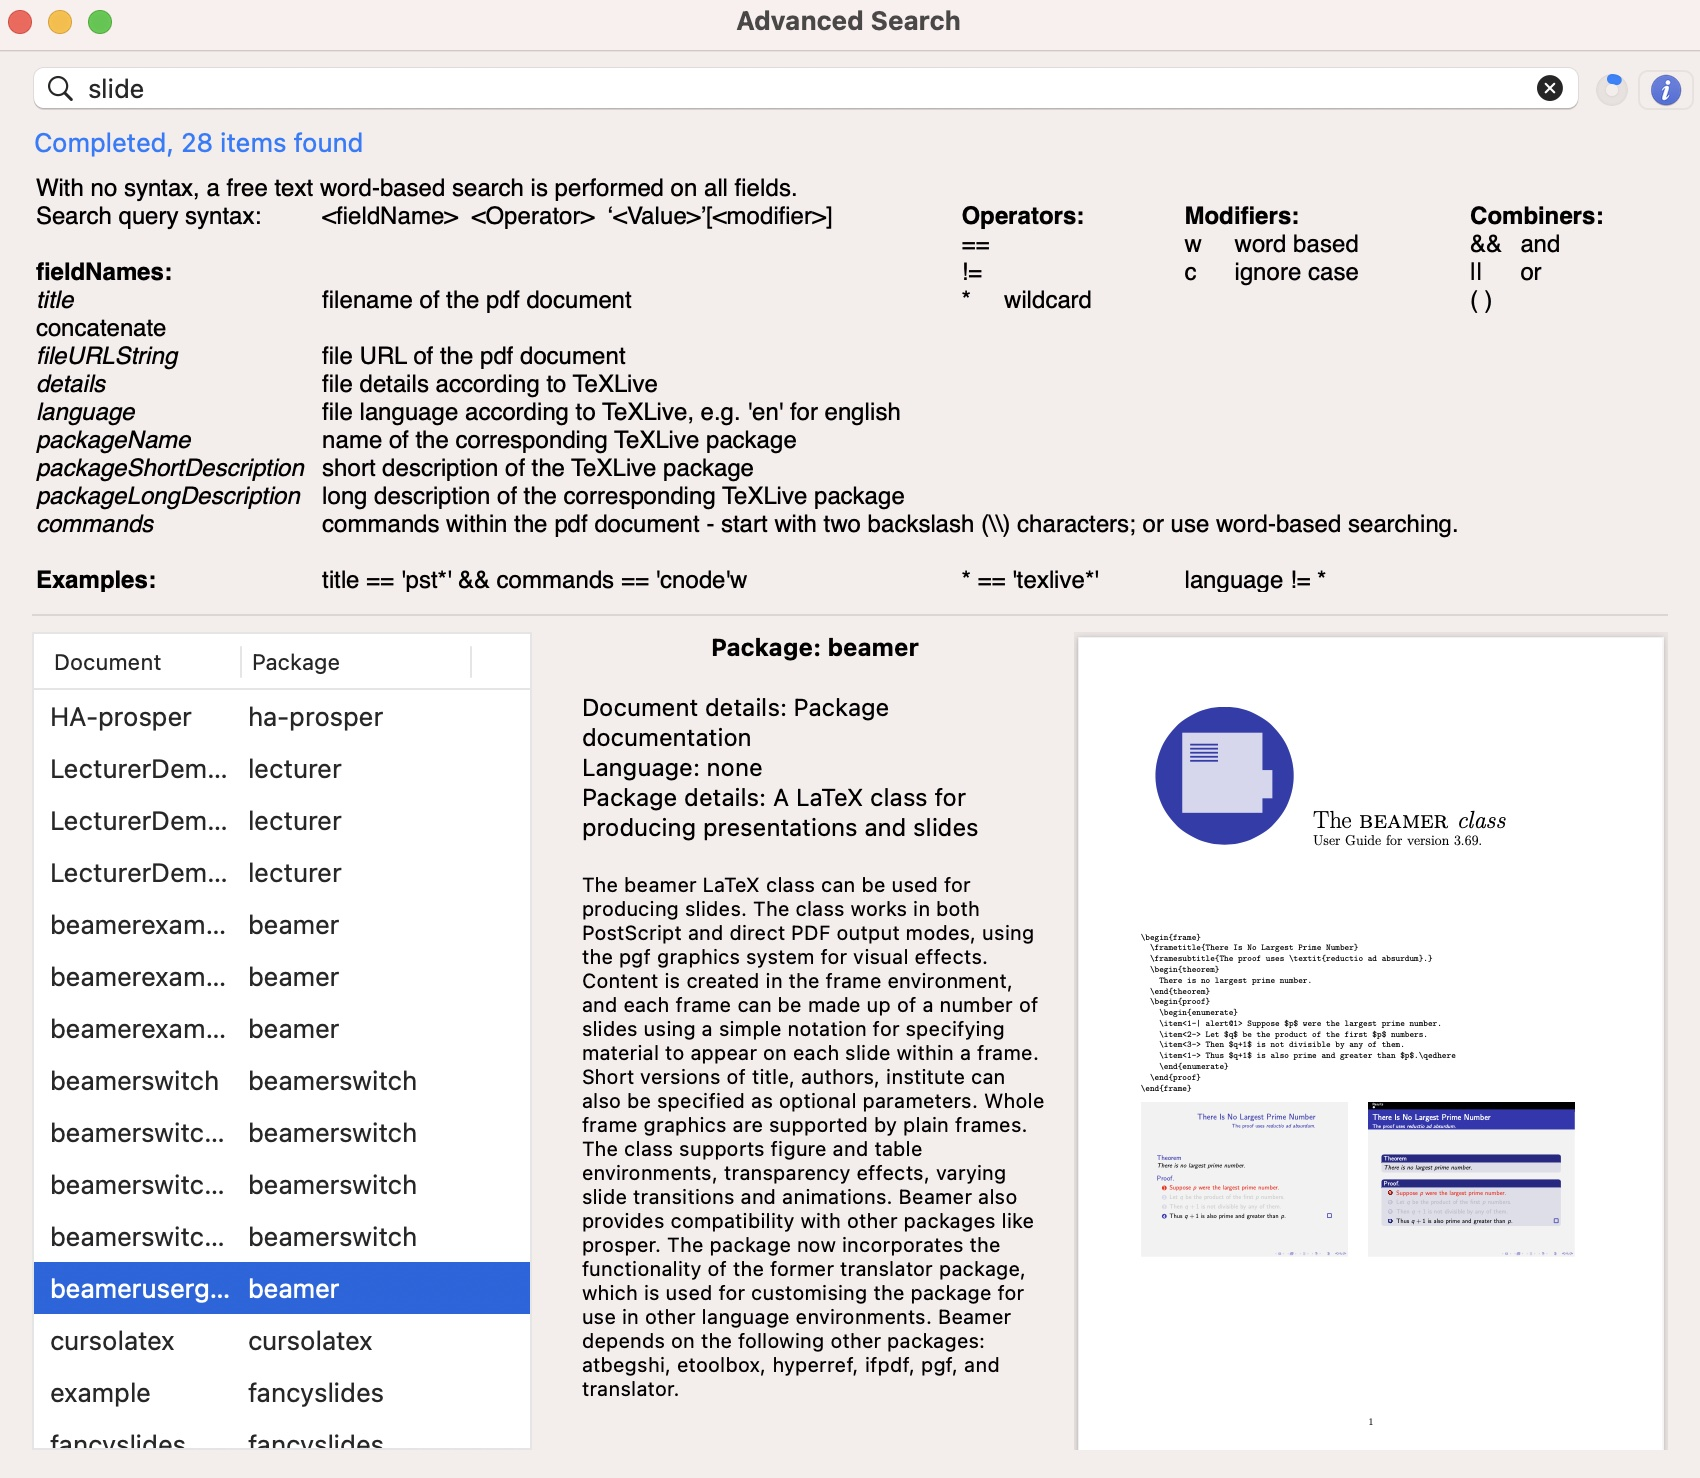
\includegraphics[scale=0.25]{AdvancedSearch.jpg}

Double-clicking on a search result opens the Help Document window.
\newpage
\section{Help Document Window}
The usual pdf-viewing commands are available along with the built-in (Preview.app) context menus. However, the left menu also provides a list of the indexed \LaTeX commands that were found within the pdf file. This only appears for files that had `Index All' enabled (see Settings). Single-clicking a command will navigate to the page where this command was most commonly found. 

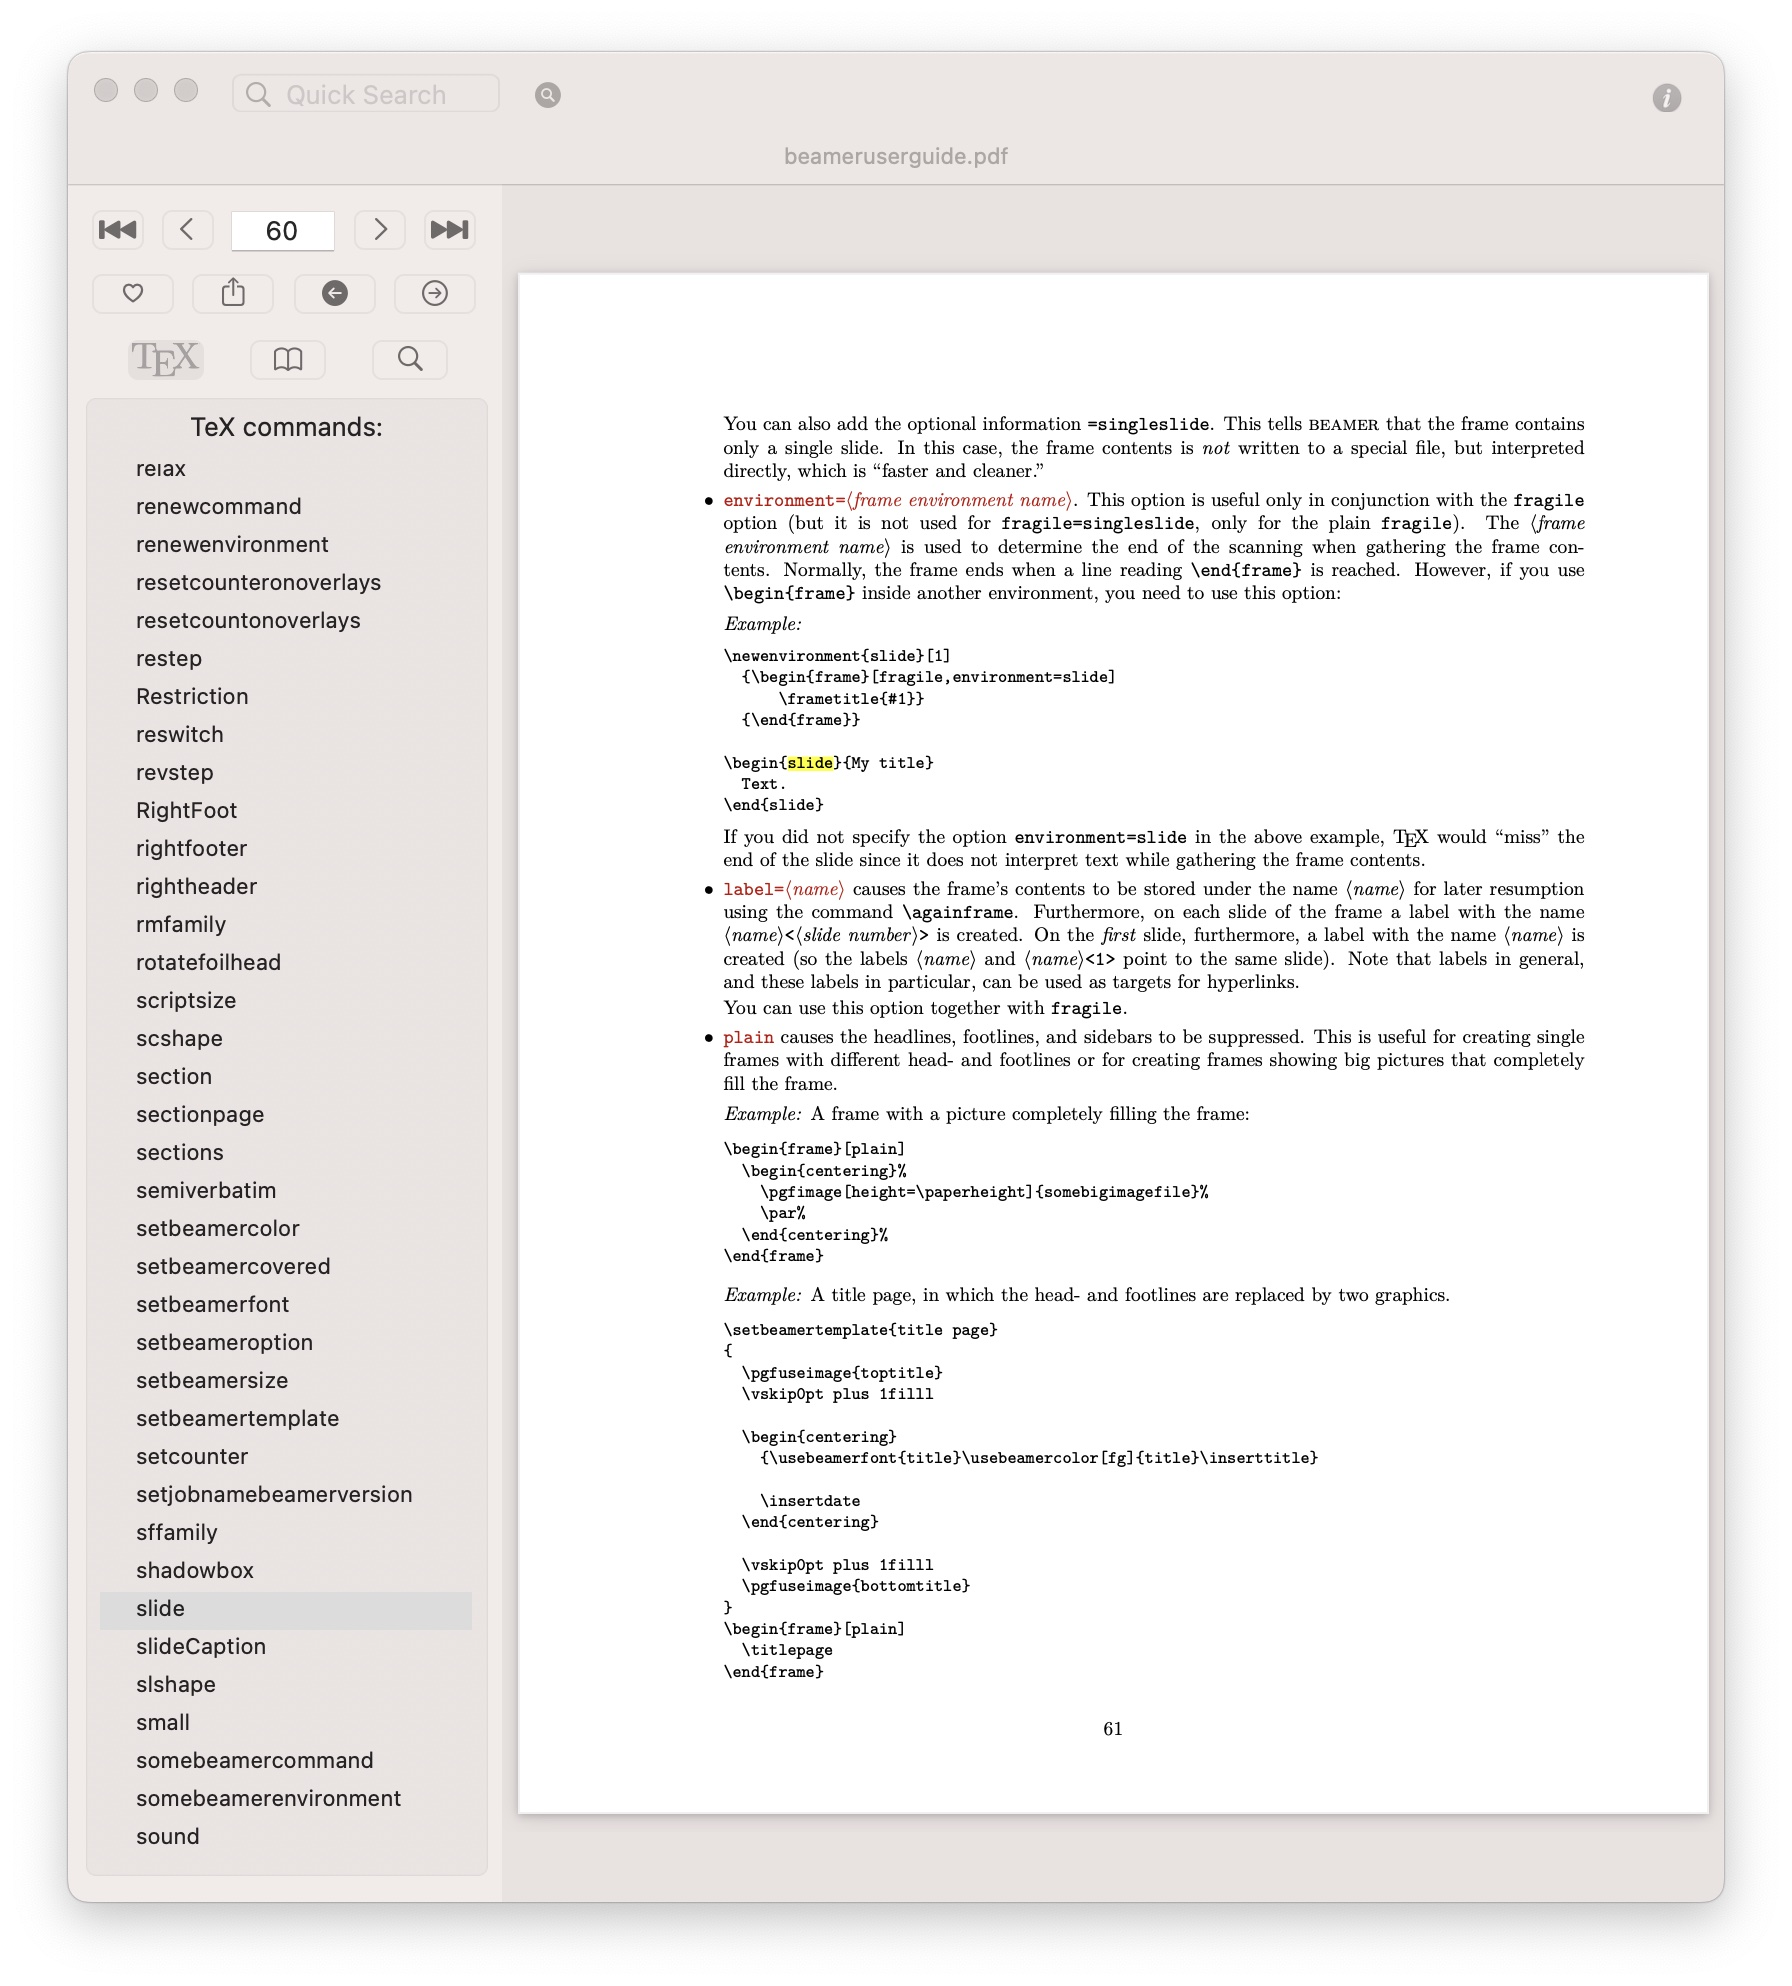
\includegraphics[scale=0.2]{HelpDoc.jpg}

Double clicking a command brings up a more detailed search result, and the other tabs reveal a normal search interface and the pdf bookmarks:

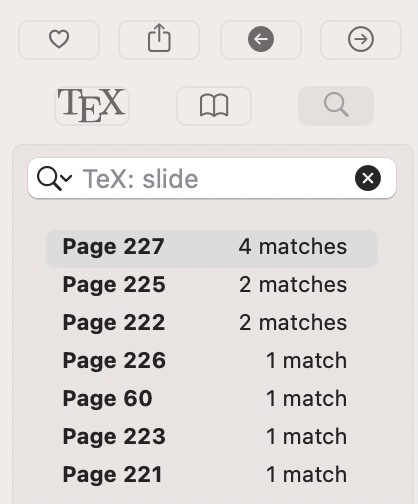
\includegraphics[scale=0.2]{TeXCommandSearch.jpg} 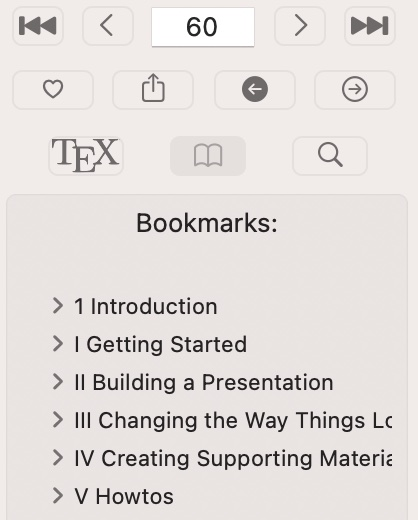
\includegraphics[scale=0.2]{Bookmarks.jpg}

Finally, the search bar at the top of the Help Document Window provides a quick search interface to look for other documents:

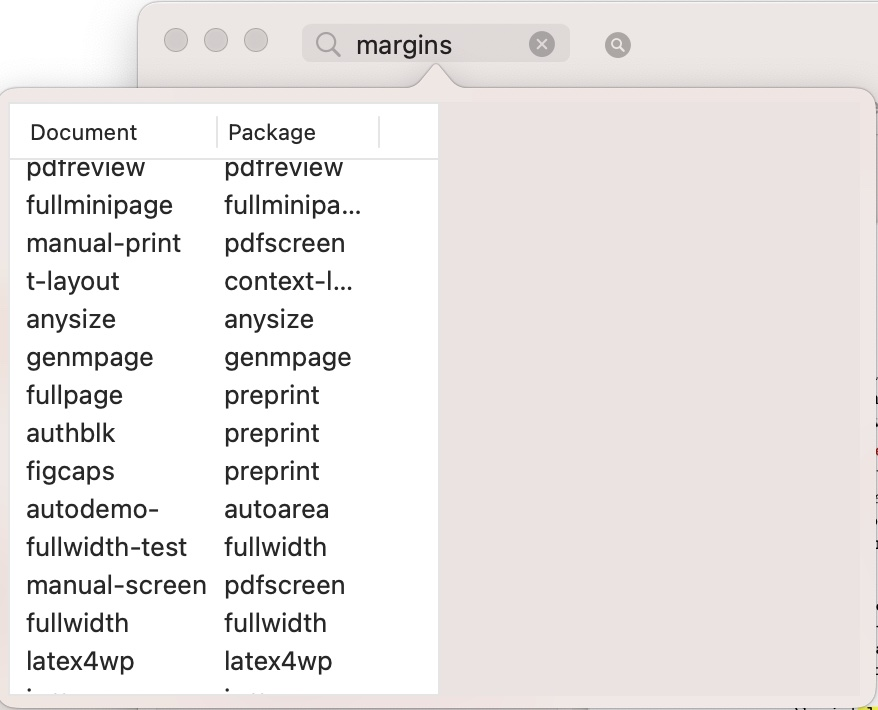
\includegraphics[scale=0.25]{QuickSearch.jpg}

\section{Settings}

\TeX Live ships with an extensive number of help documents in pdf format. Not all of these directories will be useful for all users, so the settings window allows customisation of the search. 
For `Index File Info' directories, only the package information is stored in the database. This makes indexing the database faster, and reduces the database size. 
For `Index All' directories then the pdf file contents are also searched, and an attempt is made to identify \TeX commands that might feature within the pdf document. This is not perfect, but provides a means of searching the documentation for specific commands, without knowing which package they reside in. 
Finally, with so many files in the \TeX Live distribution, there is no guarantee that all the pdf documents will be searchable (or even open-able) by the built-in pdf engines. Therefore, the indexer will automatically add files the `Excluded files' list as the indexing is performed. 

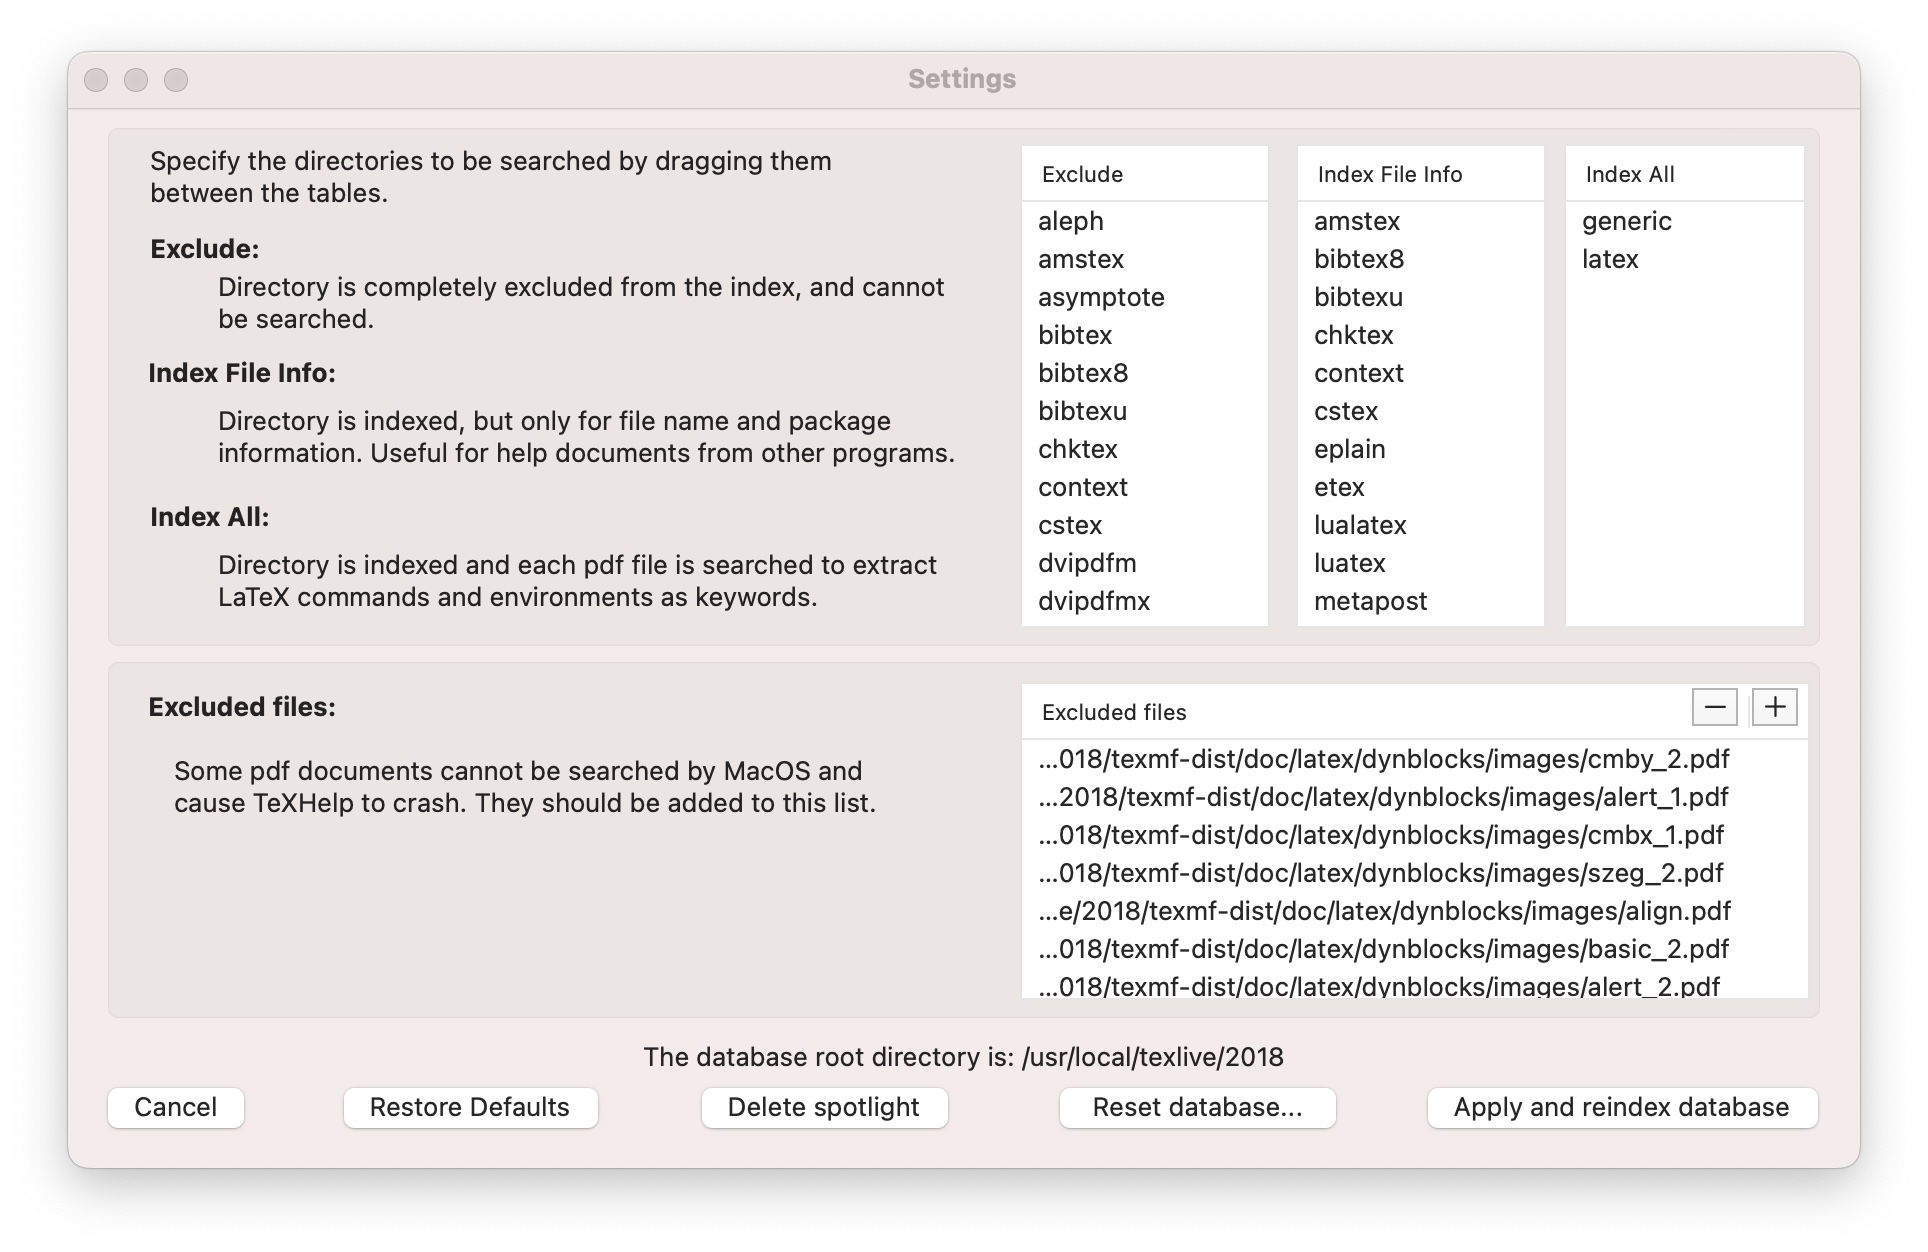
\includegraphics[scale=0.2]{Settings.jpg}
\newpage
Various configuration commands are available:
\begin{itemize}
\item `Restore Defaults' will reset the lists of excluded / included directories, and the excluded files, to the factory settings. 
\item `Delete spotlight' will remove all the database entries that are within the built-in Spotlight index. This is sometimes helpful if there is a problem with searching.
\item `Reset database' will remove the entire database (as well as the spotlight index). This allows a new database to be generated, for example based upon a different \TeX Live distribution.
\item `Apply and reindex database' simply applies any changes made to the include/exclude lists, and re-initiates indexing.
\end{itemize}

\section{File Locations}

\TeX Help stores its database in the User's Library/Containers/com.TeXHelp.TeXHelp folder. This appears as Library/Containers/TeXHelp in Finder. Within an Application Support subfolder, an sqlite database is generated. For the default settings on \TeX Live 2023, this requires about 370MB of storage. Within a Preferences subfolder, three plist files are used to save the configuration. All other files are within the TeXHelp.app. 

\section{Algorithm}
\TeX Help uses the MacOS built-in capabilities wherever possible. In particular: AppKit (for the user interface), PDFKit (for pdf searching and presentation), Core Data (for storing the database), and Core Spotlight (for searching the database). \TeX Help is written in Swift and the source files are available at \url{https://github.com/ndsims/TeXHelp.git}
\end{document}  